\begin{figure}
	\centering
	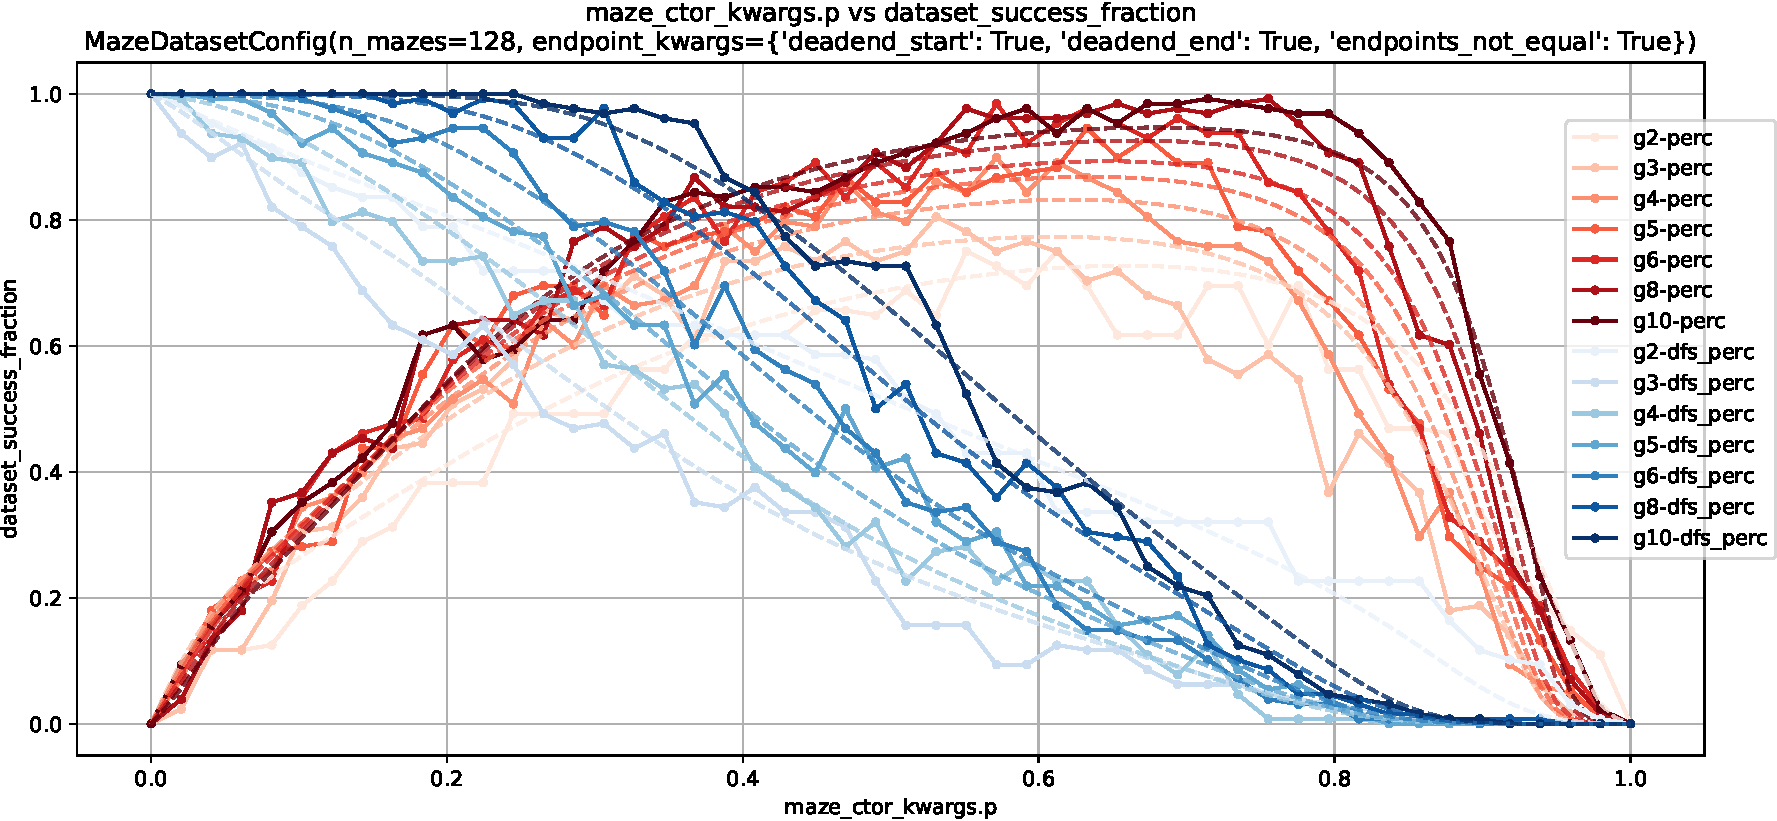
\includegraphics[width=1\textwidth,height=\textheight]{figures/ep/ep_deadends_unique-crop.pdf}
	\caption{An example of both empirical and predicted success rates as a
	function of the percolation probability \(p\) for various maze sizes,
	percolation with and without depth first search, and
	\texttt{endpoint\_kwargs} requiring that both the start and end be in
	unique dead ends. Empirical measures derived from a sample of 128 mazes.
	More information can be found on the
	\href{https://understanding-search.github.io/maze-dataset/benchmarks/}{benchmarks
	page}.}
\end{figure}